% Section content template for individual Educative lessons
% This file contains the actual content for a specific section
% Generated from Educative API section content

% Section: Requirements of Twitter’s Design
% Section ID: 5920537112477696
% Section Slug: requirements-of-twitters-design
% Generated: 2025-12-08T12:06:00.785024

\subsection{Requirements}\label{t4kblnfka5B-Fc2pR0M1A}
\\
Let's understand the functional and non-functional requirements below:

\subsubsection{Functional requirements}\label{WrHxbEwDVUFx-FVkwWfHV}
\\
The following are the functional requirements of Twitter:

\begin{itemize}
\item
\protect\phantomsection\label{Kp3qCutjw1eVNDfDVLn3i}
\textbf{Post Tweets}: Registered users can post one or more Tweets on Twitter.
\item
\protect\phantomsection\label{rPN-7rBJ6Fyy-b-0XjmeF}
\textbf{Delete Tweets}: Registered users can delete one or more of their Tweets on Twitter.
\item
\protect\phantomsection\label{trkF6YR4ITDOBPuhJClfC}
\textbf{Like or dislike Tweets}: Registered users can like and dislike public and their own Tweets on Twitter.
\item
\protect\phantomsection\label{8izm0x2M5T6MmSqwWrbU-}
\textbf{Reply to Tweets}: Registered users can reply to the public Tweets on Twitter.
\item
\protect\phantomsection\label{_DWwQJNz23NskvICXo2qD}
\textbf{Search Tweets}: Registered users can search Tweets by typing keywords, hashtags, or usernames in the search bar on Twitter.
\item
\protect\phantomsection\label{f7h65JlxC9KoI3UUVjXpO}
\textbf{View user or home timeline}: Registered users can view the user's timeline, which contains their own Tweets. They can also view the home's timeline, which contains followers' Tweets on Twitter.
\item
\protect\phantomsection\label{xAsiDOkw7I50ZTGnxAMhB}
\textbf{Follow or unfollow the account}: Registered users can follow or unfollow other users on Twitter.
\item
\protect\phantomsection\label{Lbx2VmQEw_X2M6V_gL9TA}
\textbf{Retweet a Tweet}: Registered users can Retweet public Tweets of other users on Twitter.
\end{itemize}

\subsubsection{Non-functional requirements}\label{3jyA9PdMZUnSYLCoZUohY}

\begin{itemize}
\item
\protect\phantomsection\label{WqWI-tQvMnEwC6vT8FJa_}
\textbf{Availability}: Many people and organizations use Twitter to communicate time-sensitive information (service outage messages). Therefore, our service must be highly available and have a good uptime percentage.
\item
\protect\phantomsection\label{fcVcTu7Uq04AWY99UkoHq}
\textbf{Latency}: The latency to show the most recent top Tweets in the home timeline could be a little high. However, near real-time services, such as Tweet distribution to followers, must have low latency.
\item
\protect\phantomsection\label{EjY1opUk-wmxfU7cTr2I1}
\textbf{Scalability}: The workload on Twitter is read-heavy, where we have many readers and relatively few writers, which eventually requires the scalability of computational resources. Some estimates suggest a 1:1000 write-to-read ratio for Twitter. Although the Tweet is limited to 280 characters, and the video clip is limited to 140s by default, we need high storage capacity to store and deliver Tweets posted by public figures to their millions of followers.
\item
\protect\phantomsection\label{p0JqGyEXgCOGJSo4mQ9Wm}
\textbf{Reliability}: All Tweets remain on Twitter. This means that Twitter never deletes its content. So there should be a promising strategy to prevent the loss or damage of the uploaded content.
\item
\protect\phantomsection\label{7eRXwos6UWb-AL60BF69H}
\textbf{Consistency}: There's a possibility that a user on the east coast of the US does not get an immediate status (like, reply, and so on.) update on the Tweet, which is liked or Retweeted by a user on the west coast of the US. However, the user on the west coast of the US needs an immediate status update on his like or reply. An effective technique is needed to offer rapid feedback to the user (who liked someone's post), then to other specified users in the same region, and finally to all worldwide users linked to the Tweet.
\end{itemize}

\begin{figure}[htbp]
 \centering
 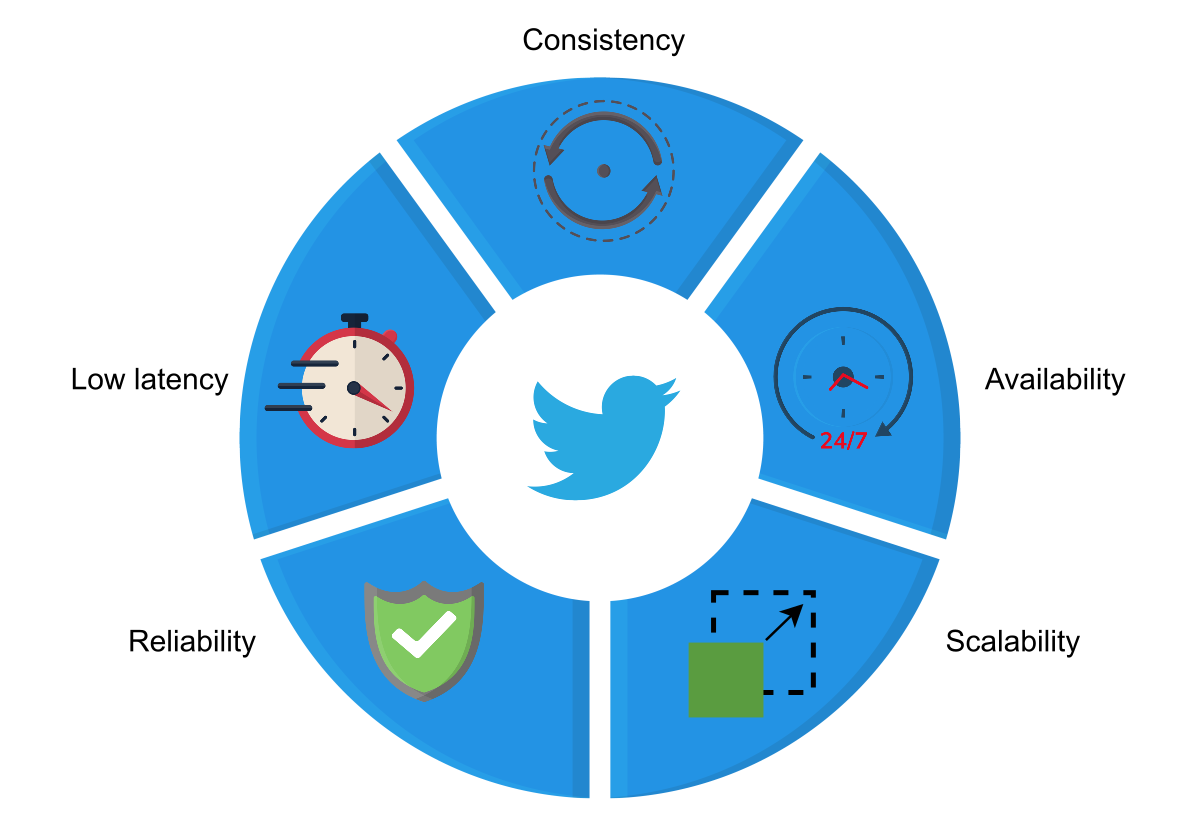
\includegraphics[width=0.5\textwidth]{Images/chapter_31/section_5920537112477696/6366079924568064.png}
 \caption{Non-functional requirements of Twitter}
\end{figure}

Furthermore, we must identify which essential resources must be estimated in the Twitter design. We used Twitter as an example in our \href{https://www.educative.io/courses/grokking-the-system-design-interview/put-back-of-the-envelope-numbers-in-perspective}{Back-of-the-Envelope} chapter, so we won't repeat the resource estimation exercise here.

\begin{figure}[htbp]
 \centering
 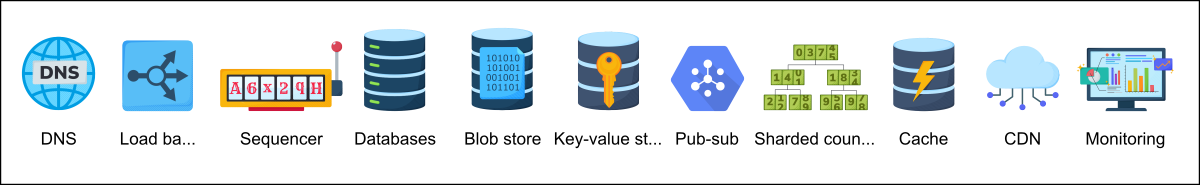
\includegraphics[width=0.5\textwidth]{Images/chapter_31/section_5920537112477696/6124993136427008.png}
 \caption{Building blocks used in Twitter design}
\end{figure}

\begin{itemize}
\item
\protect\phantomsection\label{gOQ-rBsNae55D2E86HNVA}
\href{https://www.educative.io/courses/grokking-the-system-design-interview/introduction-to-domain-name-system-dns}{\textbf{DNS}} is the service that maps human-friendly Twitter domain names to machine-readable IP addresses.
\item
\protect\phantomsection\label{jVWglwvm8hI3TvsgdIwwu}
\href{https://www.educative.io/courses/grokking-the-system-design-interview/introduction-to-load-balancers}{\textbf{Load balancers}} distribute the read/write requests among the respective services.
\item
\protect\phantomsection\label{xDMlQ6yyRcOlNTTEt5qDH}
\href{https://www.educative.io/courses/grokking-the-system-design-interview/system-design-sequencer}{\textbf{Sequencers}} generate the unique IDs for the Tweets.
\item
\protect\phantomsection\label{NwGKVKzdbnQ4gUidWvhVa}
\href{https://www.educative.io/courses/grokking-the-system-design-interview/introduction-to-databases}{\textbf{Databases}} store the metadata of Tweets and users.
\item
\protect\phantomsection\label{3DHFqfze4ywv4yI84NUEL}
\href{https://www.educative.io/courses/grokking-the-system-design-interview/system-design-a-blob-store}{\textbf{Blob stores}} store the images and video clips attached with the Tweets.
\item
\protect\phantomsection\label{ujx0Q95E7qBe_okV98ruX}
\href{https://www.educative.io/courses/grokking-the-system-design-interview/system-design-the-key-value-store}{\textbf{Key-value stores}} are used for multiple purposes such as indexing, identifying the specified counter to update its value, identifying the Tweets of a particular user and many more.
\item
\protect\phantomsection\label{vdNUfz8lFB04zkyH0D70H}
\href{https://www.educative.io/courses/grokking-the-system-design-interview/system-design-the-pub-sub-abstraction}{\textbf{Pub-sub}} is used for real-time processing such as elimination of redundant data, organizing data, and much more.
\item
\protect\phantomsection\label{wW3A_FfnDie6oACdUtI_w}
\href{https://www.educative.io/courses/grokking-the-system-design-interview/system-design-the-sharded-counters}{\textbf{Sharded counters}} help to handle the count of multiple features such as viewing, liking, Retweeting, and so on,. of the accounts with millions of followers.
\item
\protect\phantomsection\label{CDy1lAqNt5ruD2Ah65lvU}
A \href{https://www.educative.io/courses/grokking-the-system-design-interview/system-design-the-distributed-cache}{\textbf{cache}} is used to store the most requested and recent data in RAM to give users a quick response.
\item
\protect\phantomsection\label{wSixINeMCJilLZSiUAOpm}
\href{https://www.educative.io/courses/grokking-the-system-design-interview/system-design-the-content-delivery-network-cdn}{\textbf{CDN}} helps end users to access the data with low latency.
\item
\protect\phantomsection\label{HRxTAprhgEy8jIDqP1Mob}
\href{https://www.educative.io/courses/grokking-the-system-design-interview/system-design-distributed-monitoring}{\textbf{Monitoring}} analyses all outgoing and incoming traffic, identifies the redundancy in the storage system, figures out the failed node, and so on.
\end{itemize}
\\
In the next lesson, we'll discuss the design of the Twitter system.

% End of section content